% vim:ts=4:sw=4
% Copyright (c) 2014 Casper Ti. Vector
% Public domain.

\chapter{引言}
\section{背景分析}
随着网络和移动设备普及,人们越来越多的用移动设备来进行自己的社交活动,现在层出不穷的社交类应用一种在涌现,更为显著的是wechat其生态圈已经成为了中国用户一种特定的生活模式,所以移动应用在人们社交关系中起到的作用不言而喻。
并且在这个信息爆炸时代下,由于大量的信息涌到人们眼前,而不断兴起的社交媒体更是进一步将信息碎片化。不像文字一般,照片、图像作为不易切割的单位在传递信息过程中备受用户青睐。而图片类社交应用因为其独特性而成为了新一代移动应用规定的一个热点,比如国外的instagram就是图片分享类社交的先行者。而flickr,snapchat,乃至于现在出现在中国众多的社交应用都在充斥着人们的生活。甚至有人断言到“分享相片是社交网络的将来”。

% \begin{figure}[thbp!]
% \centering
% \begin{minipage}[t]{0.1\textwidth}
% \centering
% \includegraphics[width=1cm,height=1cm]{img/chap1/instagram.png}
% \caption{清明}
% \end{minipage}

% \begin{minipage}[t]{0.4\textwidth}
% \centering
% \includegraphics[width=1cm,height=1cm]{img/chap1/flickr.png}
% \caption{反复}
% \end{minipage}


% \begin{minipage}[t]{0.7\textwidth}
% \centering
% 
\includegraphics[width=1cm,height=1cm]{img/chap1/Snapchat.png}
% \caption{反复}
% \end{minipage}
% \end{figure}


\begin{figure}[h] 
\begin{minipage}[t]{0.3\linewidth}
\centering
\includegraphics[width=\textwidth]{img/chap1/flickr.png}
\caption{flickr \label{flickr}}
\end{minipage}
\hfill
\begin{minipage}[t]{0.3\linewidth}
\centering
\includegraphics[width=\textwidth]{img/chap1/instagram.png}
\caption{instagram\label{instagram}}
\end{minipage}
\begin{minipage}[t]{0.3\linewidth}
\centering
\includegraphics[width=1.2cm,height=1.2cm]{img/chap1/snapchat.png}
\caption{snapchat\label{snapchat}}
\end{minipage}

\end{figure}

但与以往社交应用类似的是大多数的图片类社交应用要么是熟人社交圈或者弱关系社交圈。而在这种关系社交类应用中,存在着用户难以找到令他们感兴趣的用户。如今的社交应用都在尝试不同的方式帮助用户去寻找他们感兴趣的用户。比如微信的“摇一摇”或者“漂流瓶”是一种具有随机性的方式,但除了一部分特定的人群,大部人的接受度并不高。而基于地点联系的方式,很多社交应用都为用户设置了查看附近的人,但使用这项功能的人并不是很多。而基于用户的兴趣,在类似于twitter,weibo这种弱关系社交中,根据关注人的和用户的某些特性,推荐好友的功能,这给予了用户一个很好的体验。而在如今的classfication中,deepwalk[引用],line[引用,张铭的论文]深度学习等算法都是未来根据用户关系来帮助用户去寻找他们感兴趣的人。

\begin{figure}[h] 
\begin{minipage}[t]{0.45\linewidth}
\centering
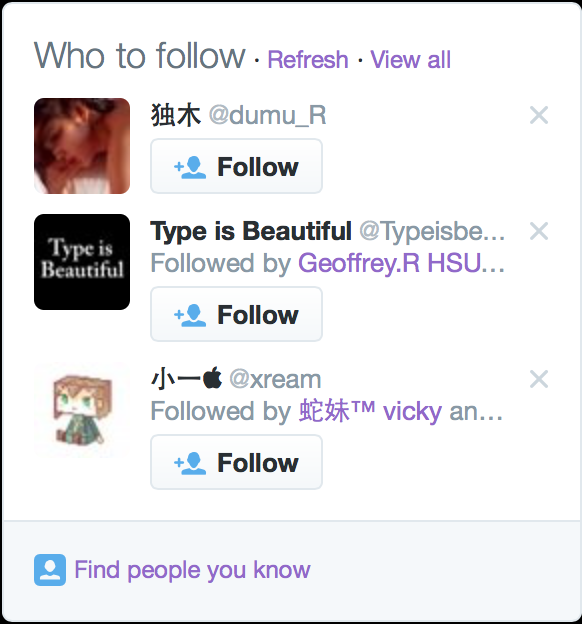
\includegraphics[width=\textwidth]{img/chap1/twitter_recommend.png}
\caption{flickr \label{Twitter推荐}}
\end{minipage}
\hfill
\begin{minipage}[t]{0.45\linewidth}
\centering
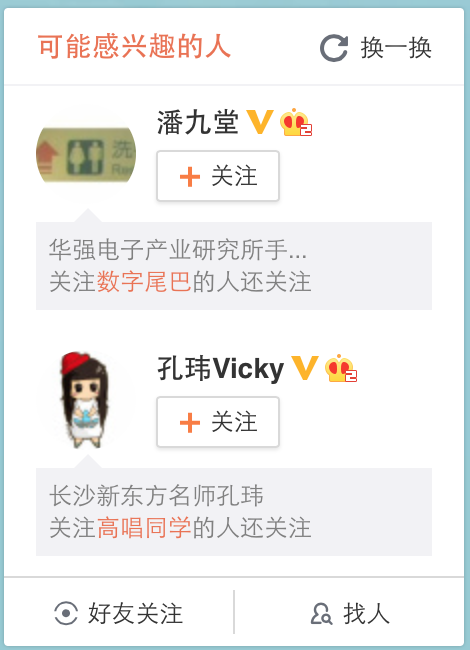
\includegraphics[width=\textwidth]{img/chap1/weibo_recommend.png}
\caption{instagram\label{weibo推荐}}
\end{minipage}

\end{figure}
虽然现在的方式各种各样,但无可否认的是至今不存在一种很好的方式提供给用户去拓展他们的社交圈子。

这就产生了本研究的一个最初的动机:能否通过一种图片交流的方式提供图片类应用的用户去认识新朋友的渠道?

而最近由于人脸识别技术的火热,市面上不断在涌现着与人脸识别关系密切的应用,比如face++与阿里巴巴在支付宝上联合推出的“刷脸”支付功能。

这些给予了笔者以灵感,笔者拟应用人脸的特征去提供一种独特的方式给用户去拓展他们的社交圈子,结合了传统的“夫妻脸“的概念,其中最基础的方式就是以人脸相似度去实现一个应用。之后通过实验的不断调整,加入其他特征去调整最后的匹配算法,得出最后的适合用户的匹配好友算法。
\section{主要研究任务}
􏰉􏴳􏰭􏴴􏴵􏴶􏴷􏰿􏴸􏴹􏴘􏰏􏲦􏲜􏱲􏴺􏰭􏴻􏲆􏴻􏴼􏰏􏱦􏴷􏱜􏰒􏴽􏳯􏴾􏴿􏵀􏱾􏱜本研究主要的任务是对于图片社交应用的一种基于人脸识别方式的好友扩展方式的研究,为用户一个良好的方式去扩展他们的社交圈。
因此本研究的主要工作总结如下:
\begin{enumerate}
\item 
\item 
\item 在移动平台上应用

\end{enumerate}
\section{研究的目的和意义}
\section{本文组织}
第一章包括背景和对研究的分析,及本文组织。第二章介绍论文相关技术和工作。第三章详细给出系统的算法和逻辑设计。第四章详细给出详细的系统的算法的。第五章进行总结和未来工作。
% 中文测试文字。
% \pkuthssffaq%

